\section{Introduction}
\label{sec:intro}

Mixture-of-Experts (MoE) architectures~\cite{jiang2024mixtral,masoudnia2014mixture,wang2025hmoe} let large language models (LLMs) scale parameter capacity without proportionally scaling per-token compute by activating only a small subset of experts per token~\cite{shazeer2017outrageously}. Designs like Switch Transformer~\cite{fedus2022switch}, GShard~\cite{lepikhin2020gshard}, and DeepSeek-V2~\cite{deepseekai2024deepseekv2strongeconomicalefficient} have made this routine. In latency-sensitive serving, however, MoE inference exposes a distinct systems bottleneck: expert weights are large, sparsely accessed, and rarely fit fully on the device, so \emph{when} and \emph{which} experts to move are as critical as routing itself.

The dominant mitigation today is \emph{cross-layer prefetching}: while executing layer~$\ell$, the runtime forecasts the experts needed by the next~$S$ MoE layers and overlaps their transfer with computation. ProMoE~\cite{song2024promoe}, ExpertFlow~\cite{he2024expertflow}, and Hobbit~\cite{tang2024hobbit} all instantiate this template; they choose the prefetch depth~$S$ \emph{offline} and reuse it across all requests. The depth itself, however, is what governs whether transfers ever land off the critical path. A too-small~$S$ leaves transfers unfinished when computation reaches layer~$\ell$, and the critical path accumulates \emph{exposed waiting latency}. A too-large~$S$ makes speculative residency exceed HBM capacity, evictions cascade, and \emph{cache pollution} amplifies subsequent miss latency. We measured this U-shaped tradeoff on three MoE models across three accelerators (\autoref{fig:M1}). At a fixed model and device, picking a sub-optimal~$S$ inflates end-to-end latency by up to $2.5\times$ as batch size changes and by up to $300\%$ as intra-batch token diversity changes (\autoref{sec:bg-motivation}). Existing fixed-horizon systems pay these inflations in full whenever the deployment differs from their tuning point.

The position of the U-shape minimum shifts with effective transfer bandwidth (a hardware property), with batch-induced contention (a workload property), and with intra-batch routing diversity (a per-request property). For any candidate offline~$S^*$, we can exhibit a workload on which some other~$S'\neq S^*$ is strictly better (\autoref{sec:bg-motivation}). Tuning~$S$ offline therefore amounts to picking the configuration on which to lose: the engineer chooses one device--workload pair on which to be optimal and accepts a multiplicative latency tax everywhere else. The right object is not a hyperparameter but a runtime control policy. A system that picks~$S_t$ at each control period in response to current stall and eviction signals can recover the wins of any fixed~$S$ \emph{simultaneously}---on the configuration where it would be best, and without offline tuning---because the controller is free to choose a different~$S$ for every (device, batch, request, layer) tuple it encounters.

We present \systemname, a serving runtime that turns the prefetch horizon~$S$ into a first-class control variable. \systemname\ has three coordinated layers (\autoref{fig:overview}(d)). A closed-loop controller updates~$S$ via a bounded $\pm 1$ rule with hysteresis on EMA-smoothed stall and eviction signals at $O(1)$ per-update cost (\autoref{sec:design:controller}). A CPU-side delta-adjusted forecaster refines pregate logits with token-, layer-, and horizon-aware features using a random forest that never touches the GPU (\autoref{sec:design:forecaster}). A residency-aware two-tier expert cache with cache-aware token routing bounds the cost of misprediction so that every prediction error costs at most one DMA, never a cascading stall (\autoref{sec:design:memory}).

\begin{figure}
    \centering
    {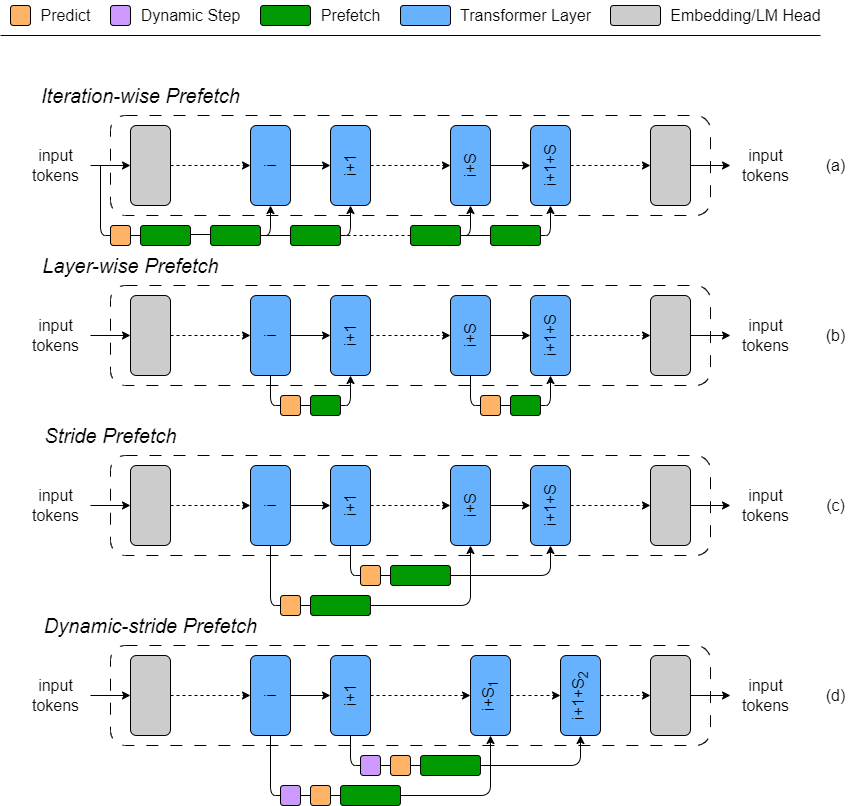
\includegraphics[width=0.99\linewidth]{figures/Candidate_prefetch_manners.png}}
    \vspace{-0.5em}
    \caption{Cross-layer expert prefetching strategies. (a)~Static
    expert--layer assignment, (b)~reactive routing, (c)~periodic
    prediction with a fixed horizon~$S$ (the template followed by
    ProMoE, ExpertFlow, and Hobbit), and (d)~\systemname's adaptive
    horizon control with feedback from runtime stall and eviction
    signals. (a)--(c) are dominated by some fixed~$S$ on every
    device--workload pair; (d) tracks the per-period optimum.}
    \label{fig:overview}
\end{figure}

We evaluate \systemname\ on NVIDIA A6000, NVIDIA H20, and Ascend 910B with DeepSeek-V2-Lite, Qwen1.5-MoE, and Qwen2-MoE under a 20\,GB HBM cap that forces expert swapping. Compared to a fixed-horizon proactive-prefetching baseline modeled after ProMoE~\cite{song2024promoe} and Eliseev~\emph{et al.}~\cite{eliseev2023fast}, \systemname\ raises expert-activation prediction accuracy by an average of $21.8\%$ (up to $30.4\%$) and reduces the cache-miss latency component by a geometric mean of $\approx 13\times$ across the eight supported model--device pairs (median $7\times$--$30\times$), while never degrading configurations in which the baseline already overlaps most transfers (e.g., Qwen2-MoE on H20). The controller's per-update cost stays under $50\,\mu$s on a commodity CPU.

We summarize our contributions as follows.
\begin{itemize}[leftmargin=1.4em, itemsep=2pt, topsep=2pt]
    \item We characterize the U-shaped overlap--pollution tradeoff of cross-layer prefetching on three MoE models and three accelerators, and show that for any candidate offline~$S^*$, the optimum lies elsewhere on some realistic workload---reframing~$S$ as a runtime control variable rather than a hyperparameter (\autoref{sec:bg-motivation}).
    \item We design a stable single-variable controller: a bounded $\pm 1$ update with hysteresis on EMA-smoothed signals tracks the per-period optimum at $O(1)$ per-update cost and is non-oscillatory by construction inside a configurable hysteresis band (\autoref{sec:design:controller}, Algorithm~\ref{alg:controller}).
    \item We co-design the forecaster and memory layer so that prediction errors are absorbed locally: a CPU-side delta-adjusted forecaster, a two-tier residency-aware cache, and cache-aware token routing together turn every prediction error into at most one DMA. We isolate the contribution of each layer via ablations on three accelerators (\autoref{sec:evaluation}).
\end{itemize}
